%Dokumentenklasse "scrbook" - Erweitert um den Verweis auf die Verzeichnisse und Texteigenschaften
\documentclass[chapterprefix=true, 12pt, a4paper, oneside, parskip=half, listof=totoc, bibliography=totoc, numbers=noendperiod]{scrbook}

% Ränder (Standard bottom ca. 52mm anbzüglich von ca. 4mm für die nach oben rechts gewanderte Seitenzahl)
%Anpassung der Seitenränder
\usepackage[bottom=48mm,left=25mm,right=25mm]{geometry}

% Ränder bei Bedarf zeigen
%\usepackage{showframe}

%Tweaks für scrbook
\usepackage{scrhack}

%Blindtext
\usepackage{blindtext}

%Erlaubt unteranderem Umbrücke captions
\usepackage{caption}

%Stichwortverzeichnis
\usepackage{imakeidx}

%Kompakte Listen
\usepackage{paralist}

%Zitate besser formatieren und darstellen
\usepackage{epigraph}

%Glossar, Stichworverzeichnis
\usepackage[toc, acronym]{glossaries} % Akronyme werden als eigene Liste aufgeführt

%Anpassung von Kopf- und Fußzeile
%beinflusst die erste Seite des Kapitels
\usepackage[automark,headsepline]{scrlayer-scrpage}
\automark{chapter}
\ihead{\leftmark}
\chead{}
\ohead{\thepage}
\ifoot*{}
\cfoot[\thepage]{}
\cfoot*{}
\ofoot*{}
\pagestyle{scrheadings}

%Auskommentieren für die Verkleinerung des vertikalen Abstandes eines neuen Kapitels
%\renewcommand*{\chapterheadstartvskip}{\vspace*{.25\baselineskip}}

%Zeilenabstand 1,5
\usepackage[onehalfspacing]{setspace}

%Verbesserte Darstellung der Buchstaben zueinander
\usepackage[stretch=10]{microtype}

%Deutsche Bezeichnungen für angezeigte Namen (z.B. Innhaltsverzeichnis etc.)
\usepackage[ngerman]{babel}

%Unterstützung von Umlauten und anderen Sonderzeichen (UTF-8)
\usepackage{lmodern}
\usepackage[utf8]{luainputenc}
\usepackage[T1]{fontenc}

%Einfachere Zitate
\usepackage{epigraph}

%Verwendung von Akronymen
\usepackage[printonlyused]{acronym}

%Unterstützung der H positionierung (keine automatische Verschiebung eingefügter Elemente)
\usepackage{float} 

%Erlaubt Umbrüche innerhalb von Tabellen
\usepackage{tabularx}

%Erlaubt Seitenumbrüche mit Tabellen
\usepackage{longtable}

%Erlaubt die Darstellung von Sourcecode mit Highlighting
\usepackage{listings}

%Definierung eigener Farben bei nutzung eines selbst vergebene Namens
\usepackage[table,xcdraw]{xcolor}

%Vektorgrafiken
\usepackage{tikz}

%Grafiken (wie jpg, png, etc.)
\usepackage{graphicx}

%Grafiken von Text umlaufen lassen
\usepackage{wrapfig}

%Ermöglicht Verknüpfungen innerhalb des Dokumentes (e.g. for PDF), Links werden durch "hidelink" nicht explizit hervorgehoben
\usepackage[hidelinks,german]{hyperref}

%Einbindung und Verwaltung von Literaturverzeichnissen
\usepackage{csquotes} %wird von biber benötigt
\usepackage[style=alphabetic, backend=biber, bibencoding=ascii]{biblatex}
\addbibresource{references/references.bib}

%-------------------------------Zusätzliche Anpassungen und Modifikationen--------------------------------------------%

%Anpassung der Überschriften
\addtokomafont{disposition}{\rmfamily}

%Zusätzliche Farben
\definecolor{darkgreen}{RGB}{0,100,0}

%Umbenennungen
\renewcommand{\lstlistlistingname}{Quelltextverzeichnis}

%Pluszeichen in der Referenc beim zitieren ausblenden
\renewcommand*{\labelalphaothers}{}

%Anpassugen zur Quelltextdarstellung, kann bei Bedarf überschrieben werden (z.B. wenn unterschiedliche Sprachen zum Einsatz kommen)
\renewcommand{\lstlistingname}{Codeauszug}
\lstset{
	language=Java,
	numbers=left,
	columns=fullflexible,
	aboveskip=5pt,
	belowskip=10pt,
	basicstyle=\small\ttfamily,
	backgroundcolor=\color{black!5},
	commentstyle=\color{darkgreen},
	keywordstyle=\color{blue},
	stringstyle=\color{gray},
	showspaces=false,
	showstringspaces=false,
	showtabs=false,
	xleftmargin=16pt,
	xrightmargin=0pt,
	framesep=5pt,
	framerule=3pt,
	frame=leftline,
	rulecolor=\color{green},
	tabsize=2,
	breaklines=true,
	breakatwhitespace=true,
	prebreak={\mbox{$\hookleftarrow$}}
}

%Anpassungen für das Abkürzungsverzeichnis
\newglossarystyle{dottedlocations}{%
	\glossarystyle{list}%
	\renewcommand*{\glossaryentryfield}[5]{%
		\item[\glsentryitem{##1}\glstarget{##1}{##2}] \emph{##3}%
		\unskip\leaders\hbox to 2.9mm{\hss.}\hfill##5}%
	\renewcommand*{\glsgroupskip}{}%
}

%%Titles - Uncomment one section of titles

%%Used for titleGraduation
\makeatletter

\newcommand*{\gradeType}[1]{\gdef\@gradeType{#1}}
\newcommand*{\firstExaminer}[1]{\gdef\@firstExaminer{#1}}
\newcommand*{\secondExaminer}[1]{\gdef\@secondExaminer{#1}}
\newcommand*{\matrikelnr}[1]{\gdef\@matrikelnr{#1}}
\newcommand*{\submitDate}[1]{\gdef\@submitDate{#1}}

\renewcommand*{\maketitle}{
	\begin{titlepage}
		\newgeometry{left=2.5cm,right=2.5cm,top=9.0cm,bottom=2.5cm}
		\begin{center}
			\vfill
			{\Large \@title\par}
			\vskip 0.5cm
			{\large \bfseries Bachelor's Thesis\par}
			\vskip 0.5cm
			{\large for obtaining the academic degree\\ \bfseries \@gradeType}
			\vskip 0.5cm
			{\large at}
			\vskip 0.5cm
			{\large Beuth Hochschule für Technik Berlin\\ Department Informatics and Media VI\\ Degree Program Mediainformatics}
			\vfill
			\begin{flushleft}
				\begin{tabular}[t]{rl}
					1. Examiner and Supervisor: &\@firstExaminer\\
					2. Examiner: & \@secondExaminer\\
					\\
					Submitted by: &\@author\\
					Matriculation number: & \@matrikelnr\\
					Date of submission: & \@submitDate
				\end{tabular}
			\end{flushleft}
		\end{center}
		\restoregeometry
	\end{titlepage}
}
\makeatother
\gradeType{Bachlor of Science (B.Sc.)}
\secondExaminer{Prof. Dr. Elmar Böhler}

%%Used for titleResearchPaper
%\makeatletter

\newcommand*{\firstExaminer}[1]{\gdef\@firstExaminer{#1}}
\newcommand*{\subTitle}[1]{\gdef\@subTitle{#1}}
\newcommand*{\researchPart}[1]{\gdef\@researchPart{#1}}
\newcommand*{\matrikelnr}[1]{\gdef\@matrikelnr{#1}}
\newcommand*{\submitDate}[1]{\gdef\@submitDate{#1}}


\renewcommand*{\maketitle}{
	\begin{titlepage}
		\newgeometry{left=2.5cm,right=2.5cm,top=9.0cm,bottom=2.5cm}
		\begin{center}
			\vfill
			{\Large \@title\par}
			{\normalsize \@subTitle\par}
			\vskip 0.5cm
			{\large \bfseries Forschungsprojekt Teil \@researchPart\par}
			\vskip 0.5cm
			{\large an der}
			\vskip 0.5cm
			{\large Hochschule für Technik und Wirtschaft Berlin\\ Fachbereich Wirtschaftswissenschaften II\\ Studiengang Angewandte Informatik}
			\vfill
			\begin{flushleft}
				\begin{tabular}[t]{rl}
					Betreuer: &\@firstExaminer\\
					\\
					Eingereicht von: &\@author\\
					Matrikelnummer: & \@matrikelnr\\
					Datum der Abgabe: & \@submitDate
				\end{tabular}
			\end{flushleft}
		\end{center}
		\restoregeometry
	\end{titlepage}
}
\makeatother
%\subTitle{Ein optionaler Untertitel der Arbeit}
%\researchPart{A}

%%Used by all titles
\title{Design and Implementation of a Tool to Collect Execution- and Service-Data of Big Data Analytics Applications}
\author{Markus Lamm}
\matrikelnr{s786694}
\submitDate{06.09.2016}
\firstExaminer{Prof. Dr. Stefan Edlich}
%%End Titles

\makeindex[title=Stichwortverzeichnis, options=-s indexstyle.ist, intoc]
\indexsetup{level=\chapter*,toclevel=chapter}

\makeglossaries
\loadglsentries{glossary_and_acronyms.tex}
\setacronymstyle{long-short}

\begin{document}

\pagenumbering{alph} %fix for same identifier warning, character is not show in title
\maketitle

\pagenumbering{Roman}

\chapter*{Ackknowledgements}
\blindtext \clearpage
\chapter*{Abstract}

\blindtext \clearpage

\tableofcontents \newpage

\pagenumbering{arabic}
\chapter{Introduction}
\section{Motivation}
According to a survey in Germany, nine out of ten companies (89 percent) analyze large
volumes of data for operational decision-making processes using modern Big Data Analytics
Architectures, where 48 percent of the respondents see the greatest potential of Big Data
\cite{Bitk14}. The analysis of continuous data streams is taking up a growing importance
for companies and therefore constitutes an important factor for business success.

Collecting, storing and analyzing system and operational data of Big Data Architectures is
therefore an essential tool in order to ensure successful operation. Even though logfiles are
usefull for tracing problems in software systems, problems can be tracked and potential sources
of error can be identified much earlier by collecting and analyzing execution and service data at
runtime to describe the state of the system at a given point in time.

Due to the distributed character of Big Data Applications, where a system is composed of several
interacting components, the examination of log data is not an adequate choice to gain insight
into the entire system \cite{VanL14}.

\section{Objective}

The main goal of the thesis is the design and implementation of a software system to ingest
and  store system and operational data of Big Data Analytics Applications on the example of
the streaming frameworks Apache Flink and Apache Kafka. It should be examined which data is
available and can be collected at all, what data is relevant and how to collect from source
systems. Furhermore, the collected data must be stored in a persistence system to become
available for possible consumers like visualization applications, analytical processes or as
a data source for applications from the context of Machine Learning for example.

\section{Structure of thesis}

After a short introduction to the topics and the main goals of the present thesis in this
chapter, the Chapter 2 covers the theoretical foundations of Big Data Analytics
Applications, discusses the concept of "stream-processing" and introduces Apache Flink
and Apache Kafka as representatives of widely used stream-processing frameworks.

Chapter 3 investigates which sources for collecting data exist for Apache Flink and Kafka
and which data should be collected and stored in a persistence system regarding to its
relevance and data quality.

The requirements and the target definition of the software-system will be introduced
in Chapter 4, Chapter 5 describes the software solution by giving a detailed conceptional
overview of the software components and providing implementation details for selected items.

In chapter 6 we'll see how to setup the technical environment for the usage of the
prototype to verify the correct functionality related to the requirements defined in
Chapter 4.

The last Chapter 7 covers a conclusion and summary of the present work.

 \clearpage
\chapter{Theoretical Foundations}

After a short introduction to the terminology of Big Data, this chapter will discuss
the main characteristics of Big Data Analytics Applications and introduces the concept of
stream processing, which is one of the main characteristics of the popular streaming
frameworks Apache Flink and Apache Kafka. The underlying concepts both of these systems
and how they're used in context of Big Data Analytics will be explained at the
end of this chapter.

\section{Big Data}

According to \cite{Marz15} the term “Big Data” is a misleading name since it implies that
pre-existing data is somehow small, which is not true, or that the only challenge is the
sheer size of data, which is just one one them among others. In reality, the term Big Data
applies to information that can’t be processed or analyzed using traditional processes or
tools.

In the past decade the amount of data being created is a subject of immense growth.
More than 30,000 gigabytes of data are generated every second, and the rate of data
creation is only accelerating.\cite{Marz15}. People create content like blog posts, tweets, social
network interactions, photos, servers continuously log messages, scientists create detailed
measurements, permanently.

\begin{figure}[H]
	\centering
	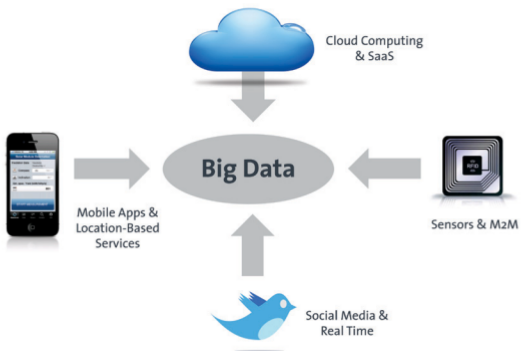
\includegraphics[width=0.7\textwidth]{../images/04-sources-of-bigdata.png}
	\caption{Sources of Big Data{\cite{Bitk12}}}
	\label{sources-of-bigdata}
\end{figure}

Through advances in communications technology, people and things are becoming in-
creasingly interconnected. Generally referred to as machine-to-machine (M2M), inter-
connectivity is responsible for double-digit year over year data growth rates. Finally,
because small integrated components are now affordable, it becomes possible to add
intelligence to almost everything. As an example, a simple railway car has hundreds
of sensors for tracking the state of individual parts and GPS-based data for shipment
tracking and logistics.\cite{Ziko12}

Besides the extremely growing amount of data, an increase in data diversity goes hand
in hand. It comes in its raw and unstructured, semistructured or structured form, which
makes processing it in a traditional relational system impractical or impossible.\cite{Bitk12}
describes, that around 85 percent of the data comes in an unstructured form, but containing
valuable information.

According to \cite{Marz15} \cite{Ziko12}, Big Data is defined by three characteristics:
\begin{description}
    \item [Volume] The amount of data present is growing because of growing amount of producers,
    e.g. environmental data, financial data, medical data, surveillance data.
    \item [Variety] Data varies in its form, it comes in different formats from different sources.
    \item [Velocity] Data needs to be evaluated and analyzed quickly, which leads to new challenges
    like analysis of large data sets with answers in seconds range, data processing in
    realtime, data generation and transmission at highspeed.
\end{description}
\begin{figure}[H]
	\centering
	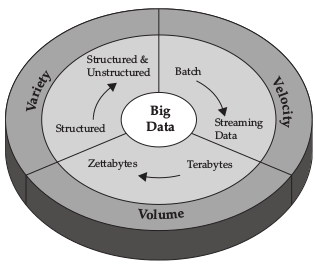
\includegraphics[width=0.7\textwidth]{../images/03-three-vs-of-bigdata.png}
	\caption{The three 'V's of Big Data{\cite{Ziko12}}}
	\label{three-vs-of-bigdata}
\end{figure}

A possible definition for Big Data could be derived as follows: \textit{Big Data refers to the use
of large amounts of data from multiple sources with a high processing speed for generating
valuable information based on the underlying data.}

\cite{Bitk12} proposes another characteristic as a fourth point called "Analytics", which will
be explained in the next section.

\section{Big Data Analytics Applications}

%Another definition comes from the the science historian George Dyson, who was cited by Tim O'Reilly in \cite{Dys13}:
%\textit{Big data is what happened when the cost of storing information became less than the cost of making the
%decision to throw it away.} It follows that the storage and extraction of valuable information from the immense amount of
%existing data has become the most important part of Big Data Analytics Applications.

Big Data Analytics describes the process of collecting, organizing and analyzing large
volumes of data with the aim to discover patterns, relationships and other useful informa-
tion extracted from incoming data streams \cite{Marz15}. The process of analytics is typically
performed using specialized software tools and applications for predictive analytics, data
mining, text mining, forecasting and data optimization.

The analytical methods raise data quality for unstructured data on a level that allows
more quantitative and qualitative analysis. With this structure it becomes posssible
to extract the data that is relevant by iteratively refined queries.

The areas of applications may be extremely diverse and ranges from analysis of financial
flows or traffic data, processing sensor data or environmental monitoring as explained in
the previous chapter.

The illustration below summarises the six-dimensional taxonomy \cite{Bitk14, Csa14} of Big
Data Analytics Applications.
\begin{figure}[H]
	\centering
	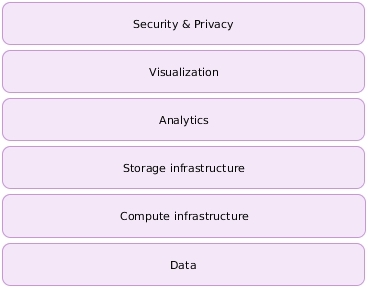
\includegraphics[width=0.7\textwidth]{../images/05-big-data-taxonomy.jpg}
	\caption{Taxonomy of Big Data Analytics Applications \cite{Bitk14, Csa14}}
	\label{taxonomy-bigdata-applications}
\end{figure}

The following section will discus the topic stream processing, which is part of the
"Compute infrastructure" layer shown in the figure above,

\section{Stream Processing}

Computing paradigms on big data currently differ at the first level of abstraction on
whether the processing will be done in batch mode, or in real-time/near real-time on
streaming data. This section is focussed on processing continous data streams in real-
time/near real-time and introduces Apache Flink and Apache Kafka as representants of
streaming frameworks.

According to \cite{Klepp16}, stream processing is the real-time processing of data continuously,
concurrently, and in a record-by-record fashion in which data is treated not as static tables
or files, but as a continuous infinite stream of data integrated from both live and historical
sources. It is needed, if “immediate” response to each event as it occurs is demanded by
the application. Various data streams could have own features. For example, a stream
from the financial market describes the whole data. In the same time, a stream for sensors
depends on sampling (e.g. get new data every 5 minutes).

The general approach is to have a small component that processes each of the events
separately. In order to speed up the processing, the stream may be subdivided, and the
computation distributed across clusters. Stream processing frameworks primarily addresses
parallelization of the computational load; an additional storage layer is needed to store
the results in order to be able to query them.

Benefits of stream processing:

\begin{itemize}
	\item Accessibility: live data can be used while still in motion, before being stored.
	\item Completeness: historical data can be streamed and integrated with live data for
	more context.
	\item High throughput: high-velocity and high-volume data can be processed with minimal latency.
\end{itemize}

In a formal way, a data stream is described as an ordered pair (S, T) where:
\begin{itemize}
	\item S is a sequence of tuples.
	\item T is a sequence of positive real time intervals.
\end{itemize}

It defines a data stream as a sequence of data objects, where the sequence in a data stream
is potentially unbounded, which means that data streams may be continuously generated
at any rate \cite{Nam15} and leads to the following characteristics:
\begin{itemize}
	\item the data arives continous
	\item the arrival of data is disorderen
	\item the size of the stream is potentially unbounded
\end{itemize}

After this short introduction to the basics of stream processing, the following sections
cover the introduction of the streaming frameworks Apache Flink and Apache Kafka and explains
the usage in the context of Big Data Analytics Applications.
\subsection{Apache Flink}

Apache Flink a framework for distributed stream and batch data processing. \cite{Flink16}

\subsection{Apache Kafka}

Apache Kafka is publish-subscribe messaging rethought as a distributed commit log. \cite{Kafka16}

%\subsection{Related work}
%
%\subsubsection{Prometheus}
%
%\subsubsection{Datadog}
%
%\subsubsection{New Relic}
%
%\subsubsection{collectd}

%collectd is a daemon which collects system performance statistics periodically and
%provides mechanisms to store the values in a variety of ways, for example in RRD files.
%
%\subsubsection{collectd}
%
%StatsD is originally a simple daemon developed and  released by Etsy  to aggregate and summarize application metrics.
%With StatsD, applications are to be instrumented by developers using language-specific client libraries. These libraries
%will then communicate with the StatsD daemon using its dead-simple protocol, and the daemon will then generate aggregate
%metrics and relay them to virtually any graphing or monitoring backend.

\section{Summary} \clearpage
%\chapter{Analysis}
%
%After a short introduction to the basic terms and Apache Flink and Apache Kafka in
%context of big data and stream processing, this chapter describes Data Quality and presents common criteria
%to measure the quality of data. Based on this criteria, available data for both of the systems will be inspected
%to build the foundation for the functional and non-functional requirements to be defined in Chapter 5 Requirements and
%Specification. The the main focus of the coming section is the analysis of available data that will be collected by the software
%solution and not a deeper exploration according to the relevance and quality of data.
%
%%In preparation of this thesis my supervisor Prof. Dr. Stefan Edlich once said \textit{"Sie sammeln
%%alles, was nicht bei drei auf dem Baum ist"}. According to this statement, the main focus
%%of the coming section is the analysis of available data that will be collected by the software
%%solution and not a deeper exploration according to the relevance and quality of data that
%%is available for Apache Flink and Apache Kafka.
%
%%\textit{"You can only control what you observe and measure."}\cite{Ebert07}. Even though logfiles, both
%%provided by Apache Flink and Apache Kafka, are usefull for tracing problems in software
%%systems, problems can be tracked and potential sources of error can be identified much
%%earlier by collecting and storing system and application data at runtime to describe the
%%state of the entire system at a given point in time.
%%
%%Due to the distributed character of Apache Flink and Apache Kafka, where a system is
%%composed of several interacting components, the examination of log data is not an
%%adequate choice to gain insight into a distributed system containing several components.\cite{VanL14}.
%%
%%Runtime data to collect can be divided in three levels of abstraction:
%%
%%\begin{enumerate}
%%    \item \textbf{Business data:} The highest level of abstraction, often refered to as Key Performance
%%    Indicators(KPI), these data expresses direct business related values and
%%    usually have very little reference to technical details. As an example, the number of
%%    sales in an online shop.
%%    \item \textbf{Application data:} On the middle level of abstraction, application data already
%%    contains many more technical details and refers to specific applications, like the
%%    number of GET requests and their corresponding HTTP Status response codes of a
%%    REST-based service.
%%    \item \textbf{System data:} The lowest level of abstraction, data provided by the underlying
%%    systems an application is running on such as cpu, memory, network, or system utilization.
%%\end{enumerate}
%%
%%Based on Apache Flink and Apache Kafka, the following section discusses the data provided
%%by both of the systems and tries a classification based on the abtraction levels.
%
%\section{System data}
%
%%System data refers to the data provided by the computer system on the lowest level of
%%abstraction and allows observation of system-related data. On unix-based systems, a
%%variety of system tools is well known to system administrators to monitor the performance
%%of servers, like vmstat (memory utilization), ifstat (network usage) or iostat (system
%%input/output) \cite{Hoeb12}.
%%
%%Another existing tool is called "DStat Versatile Resource Statistics Tool" and is described
%%as follows: \textit{"Dstat is a versatile replacement for vmstat, iostat, netstat and ifstat. Dstat
%%overcomes some of their limitations and adds some extra features, more counters and flexibility.
%%Dstat is handy for monitoring systems during performance tuning tests, benchmarks
%%or troubleshooting. Dstat allows you to view all of your system resources in real-time, you
%%can eg. compare disk utilization in combination with interrupts from your IDE controller,
%%or compare the network bandwidth numbers directly with the disk throughput (in the same
%%interval)."}\cite{Wieers16}
%%
%%Dstat is a command line tool, the following figure shows the immediate output of running
%%the application with the argument "--full", which expands more detailed information about
%%multiple cpus and network interfaces:
%%
%%\begin{figure}[H]
%%	\centering
%%	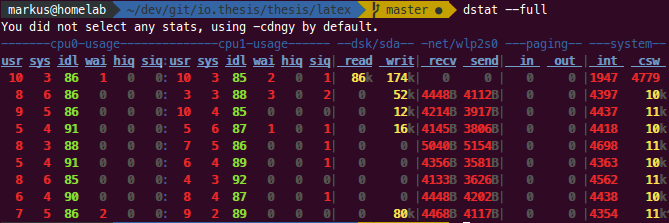
\includegraphics[width=1.0\textwidth]{../images/06-dstat-full.png}
%%	\caption{Output "dstat --full"}
%%	\label{dstat-output}
%%\end{figure}
%%
%%Additionally, Dstat provides multiple parameters to specify the data to be displayed, e.g.
%%--cpu, --disk, --net, and many more. Used in combination, the data can be grouped in the
%%following categories according to the parameters:
%%
%%\begin{table}[H]
%%    \begin{tabular}{ll}
%%        \textbf{Category} & \textbf{Dstat parameters} \\
%%        cpu & ("--cpu", "--top-cpu-adv", "--top-cputime", "--top-cputime-avg")\\
%%        disk & ("--disk", "--disk-tps", "--disk-util")\\
%%        net & ("--net", "--socket", "--tcp", "--udp")\\
%%        io & ("--io", "--top-io-adv", "--lock", "--fs")\\
%%        memory & ("--mem", "--top-mem", "--page", "--swap", "--vm")\\
%%        system & ("--sys", "--load", "--ipc", "--unix")\\
%%        process & ("--proc", "--proc-count", "--top-latency", "--top-latency-avg")\\
%%    \end{tabular}
%%    \caption{Dstat data categories}
%%    \label{tbl:dstatcategories}
%%\end{table}
%%
%%Although the parameters are mostly self-explanatory, a list containing short descriptions
%%for each of the parameter used in Chapter 4 Architecture and Implementation is available in
%%Appendix. TODO Based on the data in the extracted categories, Dstat can be considered
%%as a source that gives a fairly complete picture of the state of a system.
%%
%%Dstat is a tool only available for unix systems, and therefore not available for Windows or
%%Macintosh. Since Apache Flink and Apache Kafka are operated on Unix systems in most
%%cases, this fact can be neglected because this tool offers a wide range of data to describe
%%the system state a certain point of time.
%
%%\section{Application data}
%%
%%Every application running on the Java Virtual Machine, can be accessed via JMX as discussed
%%in Chapter 2 Basic Concepts. According the specification, every implementation of the JVM contains
%%implementations for a basic set of management interfaces, that enables the access separate parts of JVM related data,
%%located in the package "java.lang.management" \cite{Javadoc16}.
%%
%%\begin{table}[H]
%%    \begin{tabular}{ll}
%%        \textbf{Management interface} & \textbf{JMX ObjectName} \\
%%        ClassLoadingMXBean & java.lang:type=ClassLoading \\
%%        OperatingSystemMXBean & java.lang:type=OperatingSystem \\
%%        RuntimeMXBean & java.lang:type=Runtime \\
%%        ThreadMXBean & java.lang:type=Threading \\
%%        MemoryMXBean & java.lang:type=Memory \\
%%        BufferPoolMXBean & java.nio:type=BufferPool,name=* \\
%%        GarbageCollectorMXBean & java.lang:type=GarbageCollector,name=* \\
%%        MemoryManagerMXBean & java.lang:type=MemoryManager,name=* \\
%%        MemoryPoolMXBean & java.lang:type=MemoryPool,name=* \\
%%    \end{tabular}
%%    \caption{"Default" JMX JVM data}
%%    \label{tbl:jmxjvmdata}
%%\end{table}
%%
%%There's a difference in the way of data access between the object name containing an asterisk "*"
%%and the one the ones that doesn't. The asterisk indicates the existence of multiple MBeans for a given query string,
%%the result of a query for the object name "java.lang:type=GarbageCollector,name=*" results in multiple data sets according
%%to existing garbage collector names.
%%
%%This "default" set of management interfaces provides a deep insight into JVM data, is
%%available for Apache Flink and Apache Kafka and will be included in the software solution
%%in Chapter 4.
%
%\subsection{Apache Flink}
%
%Apache Flink provides application data via its monitoring API, a RESTful API, see
%Chapter 2 Basic Concepts, that delivers JSON data based on HTTP
%GET requests. It can be used to query general cluster information and status and
%statistics of running and completed jobs. The dashboard that comes with Apache Flink
%uses this monitoring API, but is designed to be used also by custom monitoring tools. The
%monitoring API runs as part of the JobManager and listens at post 8081 by default. All requests
%are of the sample form http://hostname:8081/jobs, below a list of available REST resources that
%will be used to fetch cluster- and job-related data for Apache Flink in Chapter 6 Implementation,
%see Appendix A for the corresponding JSON responses.
%
%\begin{table}[H]
%    \begin{tabular}{ll}
%        \textbf{API path} & \textbf{Description} \\
%        /config & Server setup \\
%        /overview & Cluster status \\
%        /jobs & Job ids by status running, finished, failed, canceled. \\
%        /jobs/{jobId} & Job details, dataflow plan, status, timestamps of state transitions \\
%        /jobs/{jobId}/exceptions &  Exceptions that have been observed by the job \\
%        /jobs/{jobId}/config & User-defined execution config used by the job \\
%    \end{tabular}
%    \caption{Dstat data categories}
%    \label{tbl:dstatcategories}
%\end{table}
%
%Appendix A provides a list with sample JSON response according to this REST endpoints. TODO
%
%Since version 1.1.0, Apache Flink also provides a rudimentary metrics system that exposes
%basic data for the Java Virtual Machine, the JobManagers and TaskManagers are running
%on. This data includes inter alia cpu usage or memory consumption, as well as basic
%information about running jobs. According to the "default" JVM data described in Table 3.2
%and the data provided by the monitoring REST api, the metrics system in its current version
%represents just an excerpt of the data that will be collected anyway.
%
%\subsection{Apache Kafka}
%
%In addition to the standard interfaces and MBeans that come with the implementation
%of the JVM, Apache Kafka provides a set of managed resources providing application
%specific metrics concerning the Kafka domain, reaching from global broker metrics, global
%connection metrics to metrics per topic like in- and outgoing byte rates for example. Based
%on the requirement to collect as much data as possible, the data of all provided resources
%will be collected, the complete list of MBeans observed for Apache Kafka is available in
%Appendix A.
%
%\section{Data Quality}
%
%The following covers the basics of the term "Data Quality" and examines the data sources
%introduced above based on common quality criteria.
%
%Data quality refers to the quality of data as it is provided by measurements and describes the
%ability of data to represent the mapping from an empirical system("the real world" we operate in)
%to the numeric system correctly with the main goal to satisfy a given need or objective. \cite{Ebert07}
%
%\cite{Daqua13} and  \cite{Ebert07} introduce multiple common criteria for measuring the quality of data,
%from which a selection is made to check the data previously described on their quality:
%
%\begin{enumerate}
%    \item \textbf{Correctness, Faultlessness:}
%    The data correspond to the entities of the real world, that is, the data represent the reality.
%
%    \item \textbf{Consistency:}
%    Recorded data sets does not show discrepancies, logical contradictions or errors when compared
%    among themselves.
%
%    \item \textbf{Reliability, Traceability:}
%    The origin of the data is traceable and the sources are trusted.
%
%    \item \textbf{Completeness:}
%    The required information is available and no data values are missing or in an unusable state.
%
%    \item \textbf{Accuracy:}
%    Expresses the mapping from the empirical system to the intended numerical system. Recorded values
%    conform to actual values,
%
%    \item \textbf{Timeliness:}
%    All data records correspond to the current state of the modeled world and thus are not outdated.
%    The data are the actual properties of an object from a timely manner.
%\end{enumerate}
%
%
%%
%%TODO Define DQ, evaluate quality for data above
%
%\section{Summary}
%
%According to these examinations, the following matrix of data sources results for Apache
%Flink and Apache Kafka:
%\begin{table}[H]
%\begin{tabular}{lll}
% & \textbf{Apache Flink} & \textbf{Apache Kafka} \\
%\textbf{System data (Dstat)} & X & X \\
%\textbf{JVM data (JMX)} & X & X \\
%\textbf{Application data (JMX)} & X & X \\
%\textbf{Application data (REST)} & X & - \\
%\end{tabular}
%\caption{Data source matrix}
%\label{data-source-matrix}
%\end{table}
%
%
%
%%TODO: Correlation sytem and application data
%
%In this Chapter, we discussed Dstat as a system tool that is due to its amount of available parameters
%an adequate source for retriving system data for both Apache Flink and Kafka.
 \clearpage
\chapter{Requirements}
\section{Collection}
\section{Transport}
\section{Persistence}
 \clearpage
\chapter{Architecture and Implementation}
\section{Collected data as time-series based stream}
\section{Microservices and Service-Discovery}
\section{System components}
\subsection{CollectorClient}
\subsection{CollectorManager}
\subsection{Message-Broker}
\subsection{Indexer}
\subsection{Persistence}

 \clearpage
\chapter{Test and Evaluation}
\label{ch:evaluation}
%Aufbau der Messumgebung (1­2 Seiten)
%●
%Server/Betriebssystem etc.
%Datensätze
%Anfragen
%Systeme/Ansätze gegen die Sie sich vergleichen
%Wie messen Sie? Methodik und Maßeinheiten?
%Ist die Messung signifikant?
%Hypothesen/ Was erwarten Sie?
%
%Ergebnisse und Beobachtungen (3 ­4 Seiten)
%●
%Beschreibung  der Ergebnisse
%Diagramme
%Darstellen von Zusammenhängen
%Diskussion und Bewertung (3 ­4 Seiten)
%●
%Wurden Sie überrascht?
%Stimmten Ihre Hypothesen?
%Sind Sie besser, anders als das andere System?
%Wichtigster Erkenntnisgewinn 1
%Wichtigster Erkenntnisgewinn 2
%... .
%Wichtigster Erkenntnisgewinn N
%Anwendbarkeit? Szenario?
%Zusammenfassung (ca. 0,5 Seiten)
%●
%Was haben wir in diesem Kapitel gelernt?
%Wie passt das zur Zielstellung der Arbeit
%Wie passt das zum nächsten Kapitel?
%
%In this section, we will focus on testing and evaluating implemented profiling solution. Testing
%is necessary and extremely important phase in software development lifecycle. For testing
%purposes, we have chosen several approaches:
% manual testing of chosen test scenarios,
% profiling overhead testing with for this purposes designed application,
% profiling overhead and general testing with midPoint
% Automatic testing with unit tests,
%\section{Automated test environment}

The last chapter discussed implementation details for the \textit{"Collector-Platform"} introduced in \autoref{ch:architecture}.
For its realization, Java 8 as programming language head been chosen in combination with the Spring Boot framework which allowed
the rapid implementation of self-containing, distributed applications.

In this section, the focus will be on testing and evaluating the proposed system solution to ensure compliance with the criteria
defined in \autoref{sec:fr} and \autoref{sec:nfr}.

\section{Automated Tests}

A significant approach for testing software products are automated tests that will be executed in the building process.
In Java, unit tests are used for this purpose. The \textit{Collector-Platform} uses Maven as Build-Managemement solution,
that mean the provided test implementations in form of JUnit test classes will be triggered automatically and the sucessfull passing
all existing test cases is a requirement for a successfull building process.

The \textit{"Collector-Platform"}

test
it
coverage



%Prerequisites:
%
%* [java 8](http://www.oracle.com/technetwork/java/javase/downloads/index.html)
%* [maven](https://maven.apache.org/install.html)
%* [docker](https://docs.docker.com/engine/installation/)
%* [docker-compose](https://docs.docker.com/compose/install/
%
%The application was developed and is working with the following software components:
%
%* ubuntu 16.04 LTS
%* oracle java 8
%* maven 3.3.3
%* docker 1.11.2
%* docker-compose 1.7.1

Unit- and Integration tests, IT needs docker infrastructure, usually mocked JMX, REST data,
lack of time, test separation via naming *Test and *IT via Maven Failsafe, check test coverage,
%
%5.4 Automatic Tests
%Another significant approach to testing software products are automatic tests. In java, unit tests
%are used for this purpose. We have implemented automatic tests in our solution using maven
%project management tool and TestNG framework, which provides similar functionality as
%JUnit framework with several new features.
%Scenarios in automatic tests are not that different from scenarios used in automatic
%testing. Main difference is, that in manual tests, living person needed to use applications GUI to
%perform actions defined in test scenarios, while in automatic tests, these test scenarios are
%written as standard java methods with corresponding annotations and no interaction with GUI is
%needed, we simply call specific methods to complete test scenarios (same methods are called in
%manual testing, except they are invoked by user interaction with GUI). For automatic tests, we
%also need to prepare set of test data, for example create necessary profiling objects. We can
%create them programmatically in code of current test code, or prepare them in form of XML and
%parse them during test execution.

\section{Docker environment}

local cluster
Short Docker intro, benefits in microservice environments, describe setup for components (docker-compose.yml),
describe modifications made for Apache Flink and Apache Kafka to enable JMX remote access

\begin{figure}[H]
	\centering
	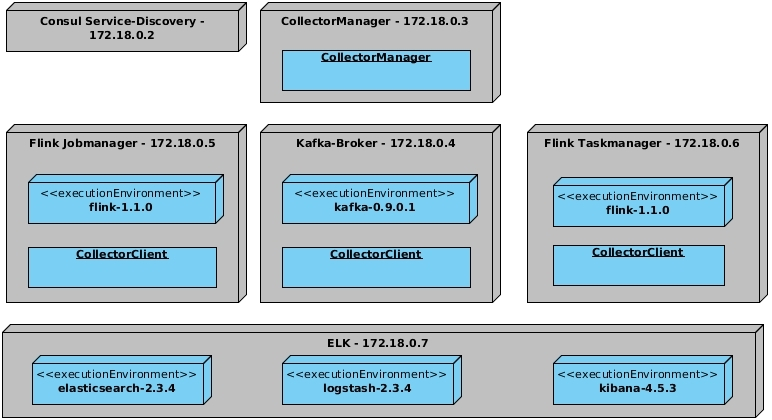
\includegraphics[width=1.0\textwidth]{../uml/deployment-diagram.jpg}
	\caption{Docker Deployment diagram}
	\label{img:deployment-diagram}
\end{figure}

Build images



%\section{Observations}
%
%CollectorDataProcessor: module to analyze the data streams creating derived streams and persist flat
%data -> data transformation, analytics layer
%
%Kibana dashboard, show visualization of CollectorDataProcessor data

\section{Discussion}
%Wurden Sie überrascht? Stimmten Ihre Hypothesen? Sind Sie besser, anders als das andere System?
%Wichtigster Erkenntnisgewinn 1
%Wichtigster Erkenntnisgewinn 2
%Wichtigster Erkenntnisgewinn N
%Anwendbarkeit? Szenario?
\section{Summary}

TODO

%Beschreibung  der Ergebnisse, Diagramme, Darstellen von Zusammenhängen \clearpage
\chapter{Conclusion}
\label{ch:conclusion}

The last chapter \autoref{ch:evaluation} presented the evaluation of the \textit{"Collector-Platform"} based on a multi node cluster
build with the Docker software container engine, that allows to run the required infrastructure components of the platform
on the local developer machine.

This last chapter summarizes the results of the previous chapters and discusses possible optimizations and alternatives to
the chosen approaches of frameworks and technologies.

\section{Summary}

The main goal of the thesis is the design and implementation of a working software system
to ingest and store data that can be collected from Apache Flink and Apache Kafka and
represents the potential data providing component for a the self-learning system, that will be developed within
germans biggest Big Data research project "Berlin Big Data Center".


%Zusammenfassung und Ausblick (5 Seiten)
%●
%●
%●
%Was lesen wir in diesem Kapitel?
%Und warum muss ich das (als Gutachter oder Interessent lesen)?
%Wie verknüpft sich dieser Inhalt mit dem vorhergehendem(n) Kapitel (n)?
%Zusammenfassung
%●
%●
%●
%●
%Was war die Zielstellung?
%Wie war unsere Vorgehensweise?
%Konnten wir das Problem/die Probleme lösen?
%Wichtigste Erkenntnisgewinne?
%Ausblick
%●
%●
%●
%Was würden Sie an dem Thema machen wenn Ihnen jetzt jemand die nächsten drei Jahre
%finanziert?
%Was würde Google / Oracle / IBM machen?
%Sollten wir eigentlich solche Dinge, die Sie in Ihrer Arbeit machen, auch wirklich erforschen
%oder bauen? Wer verliert dadurch, wer gewinnt?


\section{Outlook}

Unit-Test und Refactoring

Maybe Spring alternatives, Lagom, VertX, Play?

Maybe collector as agent, Instrumentation instead of separate service

Alternatives REST, maybe (Web-)Sockets

Possible secururity risk because remote JMX, firewalls and dstat process

More performance with more "system" languages, go? c?

dynamic sample collectors
 \clearpage

%\chapter{Beispiele} \label{c:beispiele}

Im Kapitel Beispiele (siehe \autoref{c:beispiele}) werden die möglichen Funktionen und\index{und} Möglichkeiten dies LaTeX-Dokuments demonstriert.

\section{Quelltext}

Nachfolgend der \autoref{lst:helloworld}.

\begin{lstlisting}[caption={Hello World}, captionpos=b, label={lst:helloworld}]
/**
* The HelloWorldApp class implements an application that
* simply prints "Hello World!" to standard output.
*/
class HelloWorldApp {
	public static void main(String[] args) {
		System.out.println("Hello World!"); // Display the string.
	}
}
\end{lstlisting}

\section{Bild}

\begin{wrapfigure}{R}{0.5\textwidth}
	\centering
	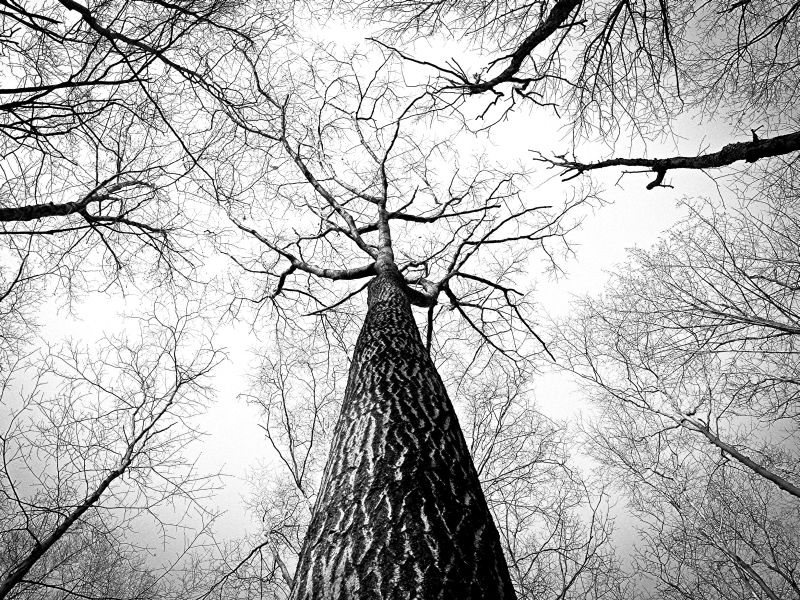
\includegraphics[width=0.5\textwidth]{resources/example}
	\caption{Beispielbild {\cite{PEXELS2015}}}
\end{wrapfigure}

Die rechts zu sehende Grafik demonstriert die Möglichkeiten des Paketes \glqq wrapfig\grqq . Grafiken innerhalb einer \glqq wrapfigure\grqq{} können entweder links oder rechts von Text umlaufen werden.

Die nachfolgende \autoref{img:beispielbild} demonstriert die Darstellung\index{Darstellung} eines \glqq *.jpg\grqq{} Bildes innerhalb des Textes (beim Einfügen kann auf die Endung verzichtet werden, solange der Name einzigartig ist). Zusätzlich enthält dieses einen Untertitel der über das bereits verwendete Label verlinkt werden kann. Der Untertitel\index{Untertitel} erscheint im \gls{abbvz}.

\section{Text Formatierungen und sonstiges}
Dieser Text enthält eine Fußnote\footnote{Fußnoten sind Anmerkungen, die im Druck-Layout aus dem Fließtext ausgelagert werden, um den Text flüssig lesbar zu gestalten.}.

\subsection{Listen}
Listen könne sowohl mit Bullet points als auch mit Zahlen erstellt werden
\begin{itemize}
	\item Eine Liste mit Bullet points
	\item Ein weiteres Element
\end{itemize}

\begin{enumerate}
	\item Eine Liste mit Zahlen
	\item Ein weiteres Element
\end{enumerate}

\subsection{Text Hervorhebungen}
\begin{quote}
	The problem with internet quotes is that you can't always depend on their accuracy \par\raggedleft--- \textup{Abraham Lincoln, 1864}
\end{quote}

"Inspirierende Zitate können mit epigraph eingefügt werden
\epigraph{The problem with internet quotes is that you can't always depend on their accuracy}{Abraham Lincoln, 1864}

Seitenumbrüche können nur direkt nach Text geschrieben werden, sonst lässt sich das Latex nicht mehr compilieren.
\\

\begin{figure}[H]
	\centering
	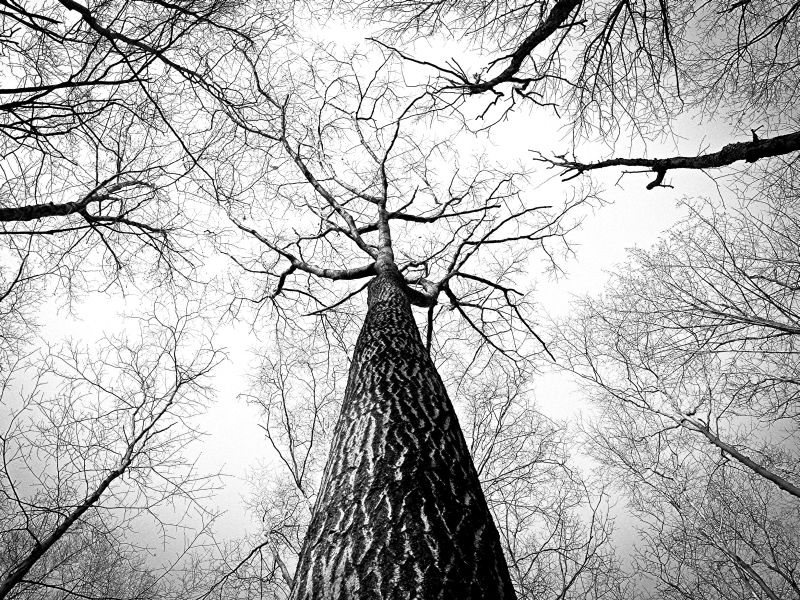
\includegraphics[width=0.7\textwidth]{resources/example}
	\caption{Beispielbild {\cite{PEXELS2015}}}
	\label{img:beispielbild}
\end{figure}

\section{Tabelle}

Nachfolgend \autoref{tbl:DigitalesZertifikat}.

\begin{table}[H]
	\begin{center}
		\renewcommand{\arraystretch}{1.3}
		\begin{tabular}{|l|}
			\hline
			\textbf{Inhaber:}\\
			Alice \\ \hline
			\textbf{Peer (Ersteller):}\\
			Bob \\ \hline
			\textbf{Öffentlicher Schlüssel des Inhabers:}\\
			F2 D2 0E ED FA 4E 9E 0A F2 DD 23 8A 32 44 F3 E9 \\ \hline
			\textbf{Gültigkeit:}\\
			2015-07-01 – 2016-06-30 \\ \hline
		\end{tabular}
	\end{center}
	\caption{Digitales Zertifikat}
	\label{tbl:DigitalesZertifikat}
\end{table}

\section{Long-Table}

Die \glqq Long-Table\grqq kann über definierte Header und Footer über Seitenumbrüche hinweg angezeigt werden.

\begin{longtable}{|l|l|l|l|}
	\hline
	\multicolumn{1}{|c}{\textbf{Version}} & \multicolumn{1}{|c}{\textbf{Codename}} &
	\multicolumn{1}{|c}{\textbf{API}} &
	\multicolumn{1}{|c|}{\textbf{Verteilung}} \\ \hline
	\endfirsthead
	
	\multicolumn{4}{c}{Fortsetzung - Verteilung der Androidversionen (Stand 01.02.2016)}\\ \hline
	\multicolumn{1}{|c}{\textbf{Version}} & \multicolumn{1}{|c}{\textbf{Codename}} &
	\multicolumn{1}{|c}{\textbf{API}} &
	\multicolumn{1}{|c|}{\textbf{Verteilung}} \\ \hline 
	\endhead
	
	\multicolumn{4}{c}{Fortsetzung auf nachfolgender Seite}
	\endfoot
	
	\caption{Verteilung der Androidversionen (Stand: 01.02.2016)}
	\label{tab:androidverteilung}
	\endlastfoot
	
	2.2 & Froyo & 8 & 0.1\%\\ \hline
	2.3.3 - 2.3.7 & Gingerbread & 10 & 2.7\%\\ \hline
	4.0.3 - 4.0.4 & Ice Cream Sandwich & 15 & 2.5\%\\ \hline
	4.1.x & Jelly Bean & 16 & 8.8\%\\ \cline{1-1} \cline{3-4}
	4.2.x &  & 17 & 11.7\%\\ \cline{1-1} \cline{3-4}
	4.3 &  & 18 & 3.4\%\\ \hline
	4.4 & KitKat & 19 & 35.5\%\\ \hline
	5.0 & Lollipop & 21 & 17.0\%\\ \cline{1-1} \cline{3-4}
	5.1 &  & 22 & 17.1\%\\ \hline
	6.0 & Marshmallow & 23 & 1.2\%\\ \hline
\end{longtable}

\section{Literaturverweis}

Weil für die alte\index{alte} und die neue Rechtschreibung verschiedene Trennregeln\index{Trennregeln} gelten, sind Deutsch mit alter Rechtschreibung und Deutsch mit neuer Rechtschreibung zwei verschiedene Sprachen (\cite{Knappen2009}, S. 192).

\section{Onlineverweise}

Siehe Google.de \cite{Google2015}.

\section{Glossar}
Der Glossar enthält die Beschreibung verwendeter Begriffe für das bessere Verständnis gegenüber dem Leser. Beispiele sind: \gls{berlin}, \gls{outsourcing}, \gls{asp}, \gls{policy} und \gls{pcie}.

\section{Abkürzungsverzeichnis}
Das Abkürzungsverzeichnis listet alle verwendeten Abkürzungen auf. Einige Beispiele sind \gls{sas}, \gls{cd}, \gls{lan} und \gls{iso}. Die erneute Verwendung zeigt nur noch die Abkürzung: \gls{sas}, \gls{cd}, \gls{lan} und\index{und} \gls{iso}. \clearpage

\pagenumbering{Alph}
\listoffigures \clearpage
\listoftables \clearpage
\lstlistoflistings \clearpage

\printindex \clearpage

\printglossary[title={Glossar}] \clearpage
\printglossary[style=dottedlocations,type=\acronymtype,title={Abkürzungsverzeichnis}] \clearpage

\printbibliography[heading=bibintoc, keyword={book}, title={Literaturverzeichnis}]\clearpage
\printbibliography[heading=bibintoc, keyword={online}, title={Onlinequellen}]\clearpage
\printbibliography[heading=bibintoc, keyword={image}, title={Bildquellen}]\clearpage

% Anhang
\appendix

\chapter{}
\addcontentsline{toc}{chapter}{Anhang A}

\section{Diagramm}

\section{Tabelle}

\section{Screenshot}

\section{Graph}

% Eigenständigkeitserklärung
\addchap{Eigenständigkeitserklärung}

Hiermit versichere ich, dass ich die vorliegende Masterarbeit selbstständig und nur unter
Verwendung der angegebenen Quellen und Hilfsmittel verfasst habe. Die Arbeit wurde bisher
in gleicher oder ähnlicher Form keiner anderen Prüfungsbehörde vorgelegt.

\vskip 1cm

Stadt, den xx.xx.xxxx

\vskip 1.5cm

Max Mustermann

\end{document}